\documentclass{article}
\usepackage{spikey}
\usepackage{amsmath}
\usepackage{mathrsfs}
\usepackage{amssymb}
\usepackage{soul}
\usepackage{float}
\usepackage{graphicx}
\usepackage{hyperref}
\usepackage{fancyhdr}
\usepackage{xcolor}
\usepackage{chngcntr}
\usepackage{centernot}
\usepackage[shortlabels]{enumitem}
\usepackage[margin=1truein]{geometry}
\usepackage{tkz-graph}
\usepackage{dsfont}
\usepackage{caption}
\usepackage{subcaption}
\usepackage[yyyymmdd,hhmmss]{datetime}

\usepackage{setspace}
\linespread{1.15}
\usepackage[margin=1truein]{geometry}

\counterwithin{equation}{section}
\counterwithin{figure}{section}

\usepackage{listings}
 
\definecolor{codegreen}{rgb}{0,0.6,0}
\definecolor{codegray}{rgb}{0.5,0.5,0.5}
\definecolor{codeblue}{rgb}{0.3,0.5,0.8}
\definecolor{codepurple}{rgb}{0.58,0,0.82}
%\definecolor{backcolour}{rgb}{0.95,0.95,0.92}
\definecolor{backcolour}{rgb}{1,1,1}

\lstdefinestyle{mystyle}{
    backgroundcolor=\color{backcolour},   
    commentstyle=\color{codegreen},
    keywordstyle=\color{magenta},
    numberstyle=\tiny\color{codegray},
    stringstyle=\color{codepurple},
    basicstyle=\ttfamily\footnotesize,
    breakatwhitespace=false,         
    breaklines=true,                 
    captionpos=b,                    
    keepspaces=true,                 
    numbers=left,                    
    numbersep=5pt,                  
    showspaces=false,                
    showstringspaces=false,
    showtabs=false,                  
    tabsize=4
}

\lstset{style=mystyle}

\title{CSC413: Programming Assignment 1}
\date{\today\ at \currenttime}
\author{Tianyu Du (1003801647)}
\begin{document}
    \maketitle
    \section{Linear Embedding GLoVE}
    \paragraph{Question 1} For each $i \in \{1, 2, \cdots, V\}$, $\vew_i \in \R^d$ and $b_i \in \R$. For each vocabulary, there are $d + 1$ corresponding trainable parameters. The total number of trainable parameters is therefore
    \begin{align}
    	V (d + 1)
    \end{align}
    
    \paragraph{Question 2}
    Define
    \begin{align}
    	\delta_{ij} &:= \vew_i^T \vew_j + b_i + b_j - \log X_{ij}
    \end{align}
    By construction, $X$ is symmetric, hence,
    \begin{align}
    	\delta_{ij} &= \delta_{ji}\quad \forall i, j
    \end{align}
    Let $\alpha \in \{1, 2, \cdots, V\}$,
    \begin{align}
    	\pd{}{\vew_\alpha} L\left(\left\{\mathbf{w}_{i}, b_{i}\right\}_{i=1}^{V}\right) 
    	&= \pd{}{\vew_\alpha} \sum_{i, j=1}^{V}\left(\mathbf{w}_{i}^{\top} \mathbf{w}_{j}+b_{i}+b_{j}-\log X_{i j}\right)^{2} \\
    	&= \pd{}{\vew_\alpha} \left[\sum_{i=j=\alpha} \delta_{ij}^2 
    	+ \sum_{i=\alpha} \sum_{j\neq\alpha} \delta_{ij}^2
		+ \sum_{i\neq\alpha} \sum_{j=\alpha}\delta_{ij}^2
		+ \sum_{i, j \neq \alpha} \sum_{j=\alpha}\delta_{ij}^2 \right] \\
		&= \pd{}{\vew_\alpha} \left[\sum_{i=j=\alpha} \delta_{ij}^2 
    	+ \sum_{i=\alpha} \sum_{j\neq\alpha} \delta_{ij}^2
		+ \sum_{i\neq\alpha} \sum_{j=\alpha}\delta_{ij}^2
		\right] \\
		&= \pd{}{\vew_\alpha}\left[ \delta_{\alpha \alpha}^2 
    	+ \sum_{j\neq\alpha} \delta_{\alpha j}^2
		+ \sum_{i\neq\alpha} \delta_{i \alpha}^2
		\right] \\
		&= \pd{}{\vew_\alpha}\left[ \delta_{\alpha \alpha}^2 
    	+ \sum_{j\neq\alpha} \delta_{j \alpha}^2
		+ \sum_{i\neq\alpha} \delta_{i \alpha}^2
		\right] \\
		&= \pd{}{\vew_\alpha}\left[ \delta_{\alpha \alpha}^2 
		+ 2 \sum_{i\neq\alpha} \delta_{i \alpha}^2
		\right] \quad (\dagger)
    \end{align}
    Because $\pd{\norm{\vew}_2^2}{\vew} = 2 \vew^T$,
    \begin{align}
    	\pd{}{\vew_\alpha} \delta_{\alpha \alpha}^2 &= 2 \delta_{\alpha \alpha} 2 \vew_\alpha^T \\
    	&= 4 \delta_{\alpha \alpha} \vew_\alpha^T
    \end{align}
    For other $i \neq \alpha$
    \begin{align}
    	\pd{}{\vew_\alpha} \delta_{i \alpha}^2 &= 2 \delta_{i\alpha} \pd{}{\vew_\alpha} \delta_{i\alpha} \\
    	&= 2 \delta_{i \alpha} \vew_i^T
    \end{align}
    Altogether with ($\dagger$),
    \begin{align}
    	\pd{}{\vew_\alpha} L\left(\left\{\mathbf{w}_{i}, b_{i}\right\}_{i=1}^{V}\right)
    	&= 4 \delta_{\alpha \alpha} \vew_\alpha^T + 2 \sum_{i \neq \alpha} 2 \delta_{i \alpha} \vew_i^T \\
    	&= 4 \sum_{i=\alpha} \delta_{i\alpha} \vew_i^T \quad(\dagger \dagger)
    \end{align}
    Taking the transpose of derivative ($\dagger\dagger$) gives the gradient
    \begin{align}
    	\nabla_{\vew_\alpha} L\left(\left\{\mathbf{w}_{i}, b_{i}\right\}_{i=1}^{V}\right)
    	&= 4 \sum_{i=\alpha} \delta_{i\alpha} \vew_i
    \end{align}
    Following the same procedure of deriving ($\dagger$), the derivative of $L$ with respect to $b_\alpha$ is:
    \begin{align}
    	\pd{}{b_\alpha} L\left(\left\{\mathbf{w}_{i}, b_{i}\right\}_{i=1}^{V}\right)
    	&= \pd{}{b_\alpha}\left[ \delta_{\alpha \alpha}^2 
		+ 2 \sum_{i\neq\alpha} \delta_{i \alpha}^2
		\right] \\
		&= 2 \delta_{\alpha \alpha} \pd{}{b_\alpha} (\norm{\vew_\alpha}^2_2 + 2 b_\alpha - \log X_{\alpha \alpha})
		+ 2 \pd{}{b_\alpha} \sum_{i \neq \alpha} (\vew_i^T \vew_\alpha + b_i + b_\alpha - \log X_{i \alpha})^2 \\
		&= 4 \delta_{\alpha \alpha} + 2 \sum_{i \neq \alpha} 2 \delta_{i\alpha} \\
		&= 4 \sum_{i=1}^V \delta_{i \alpha}
    \end{align}
    
    \paragraph{Question 3} Implementation: 
    \begin{lstlisting}[language=python]
def grad_GLoVE(W, b, log_co_occurence):
    "Return the gradient of GLoVE objective w.r.t W and b."
    "INPUT: W - Vxd; b - Vx1; log_co_occurence: VxV"
    "OUTPUT: grad_W - Vxd; grad_b - Vx1"
    V, d = W.shape
    n,_ = log_co_occurence.shape
    ###########################   YOUR CODE HERE  ##############################
    delta = (W @ W.T + b @ np.ones([1,n]) + np.ones([n,1])@b.T - log_co_occurence)
    grad_W = 2 * (delta @ W + delta.T @ W)
    grad_b = 4 * np.sum(delta, axis=1).reshape(V, 1)
	############################################################################
    return grad_W, grad_b	
    \end{lstlisting}
    
    \paragraph{Question 4} As embedding dimension increases, the performance of model firstly goes up and then down. An embedding dimension of $d=12$ leads to the optimal performance according to the validation loss. When the embedding dimension is low, increasing the dimension allows the embedding procedure to extract more meaningful information on the concurrence between words. However, when the embedding dimension is too large, the afterward neural network (the one takes embedded results and outputs the prediction) do not have enough complexity (in terms of the number of neurones) to predict next word based on high dimensional features (e.g., the dimension of features would be 150 if we are using 50d embedding).
    \begin{figure}[H]
    	\centering
    	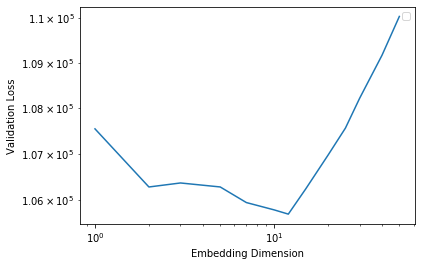
\includegraphics[width=0.7\linewidth]{performance_emb_dim.png}
    \end{figure}
    
    \section{Network architecture}
    \paragraph{Question 1} Suppose the embedding layers are already trained, and they are not trainable in this section. \\
    The \texttt{word\_embedding\_weights} has shape $16 \times 250$, which maps one-hot-vector representing identities of words to their corresponding embeddings. This weight has been trained in the previous section, therefore, possesses zero trainable parameters. Note that this layer has no bias term.\\
    The \texttt{embed\_to\_hid\_weights} maps the embedding results of three context words ($3 \times 16 = 48$ d) to the 128d hidden layer. Hence,
    \begin{align}
    	\textbf{W}_\texttt{embed\_to\_hid\_weights} \in \R^{128 \times 48} \\
    	\textbf{b}_\texttt{embed\_to\_hid\_weights} \in \R^{128}
    \end{align}
    All entries in the weight and bias are trainable. \\
    The layer with \texttt{hid\_to\_output\_weights} maps 128d hidden neurones to 250d outputs. Therefore,
    \begin{align}
    	\textbf{W}_\texttt{embed\_to\_hid\_weights} \in \R^{250 \times 128} \\
    	\textbf{b}_\texttt{embed\_to\_hid\_weights} \in \R^{250}
    \end{align}
    All entries in the weight and bias are trainable. \\
    Total number of trainable parameters is
    \begin{align}
    	128 \times 48 + 128 + 250 \times 128 + 250 = 38522
    \end{align}
    The \texttt{embed\_to\_hid\_weights} part has the largest number of trainable parameters.
    
    \paragraph{Question 2} A 4-grams requires $250^3$ possible set of context words $\vew = (w_1, w_2, w_3)$, and for each \vew, there are 250 possible following words. The total number of combinations is 
    \begin{align}
    	250^4 = 3906250000
    \end{align}
    
    \section{Training the Neural Network}
    \paragraph{Outputs} outputs from \texttt{check\_gradients} and \texttt{print\_gradients} methods.
    \begin{lstlisting}
The loss derivative looks OK.
The gradient for word_embedding_weights looks OK.
The gradient for embed_to_hid_weights looks OK.
The gradient for hid_to_output_weights looks OK.
The gradient for hid_bias looks OK.
The gradient for output_bias looks OK.
loss_derivative[2, 5] 0.001112231773782498
loss_derivative[2, 121] -0.9991004720395987
loss_derivative[5, 33] 0.0001903237803173703
loss_derivative[5, 31] -0.7999757709589483

param_gradient.word_embedding_weights[27, 2] -0.27199539981936866
param_gradient.word_embedding_weights[43, 3] 0.8641722267354154
param_gradient.word_embedding_weights[22, 4] -0.2546730202374648
param_gradient.word_embedding_weights[2, 5] 0.0

param_gradient.embed_to_hid_weights[10, 2] -0.6526990313918256
param_gradient.embed_to_hid_weights[15, 3] -0.13106433000472612
param_gradient.embed_to_hid_weights[30, 9] 0.118467746181694
param_gradient.embed_to_hid_weights[35, 21] -0.10004526104604386

param_gradient.hid_bias[10] 0.25376638738156415
param_gradient.hid_bias[20] -0.03326739163635379

param_gradient.output_bias[0] -2.0627596032173052
param_gradient.output_bias[1] 0.0390200857392169
param_gradient.output_bias[2] -0.7561537928318482
param_gradient.output_bias[3] 0.21235172051123635
    \end{lstlisting}
    \paragraph{Implementations} See the submitted Jupyter notebook file for detailed implementations.
    \begin{lstlisting}[language=Python]
def compute_loss_derivative(self, output_activations, expanded_target_batch):
	...
    ###########################   YOUR CODE HERE  ##############################
    return output_activations - expanded_target_batch  # batch_size x vocab_size
    ############################################################################
    \end{lstlisting}
    \begin{lstlisting}[language=Python]
def back_propagate(self, input_batch, activations, loss_derivative):
	...
	###########################   YOUR CODE HERE  ##############################
	hid_to_output_weights_grad = loss_derivative.T @ activations.hidden_layer
	output_bias_grad = np.sum(loss_derivative, axis=0)
	embed_to_hid_weights_grad = hid_deriv.T @ activations.embedding_layer
	hid_bias_grad = np.sum(hid_deriv, axis=0)
	############################################################################
	...
    \end{lstlisting}
    
    \section{Analysis}
    \paragraph{Question 1} The predicted probabilities can be found below. For the first example, the model predicts 'government of united \ul{own}', which does not really make sense. But for the second and third trails, the model produces sensible outputs. 
    \begin{lstlisting}
>>> trained_model.predict_next_word("government", "of", "united")
government of united own Prob: 0.06786
government of united states Prob: 0.06067
government of united life Prob: 0.05791
government of united money Prob: 0.05206
government of united . Prob: 0.05050
government of united end Prob: 0.04033
government of united time Prob: 0.03520
government of united house Prob: 0.03320
government of united say Prob: 0.02317
government of united team Prob: 0.02231

>>> trained_model.predict_next_word("city", "of", "new")
city of new york Prob: 0.98987
city of new . Prob: 0.00139
city of new ? Prob: 0.00080
city of new , Prob: 0.00078
city of new days Prob: 0.00059
city of new children Prob: 0.00058
city of new times Prob: 0.00055
city of new years Prob: 0.00033
city of new music Prob: 0.00033
city of new people Prob: 0.00030

>>> trained_model.predict_next_word("life", "in", "the")
life in the world Prob: 0.15756
life in the first Prob: 0.13498
life in the end Prob: 0.05317
life in the united Prob: 0.04379
life in the street Prob: 0.04040
life in the game Prob: 0.03705
life in the country Prob: 0.03588
life in the school Prob: 0.02934
life in the place Prob: 0.02903
life in the city Prob: 0.02711
    \end{lstlisting}
    \texttt{find\_occurrences("life", "in", "the")} returns
    \begin{lstlisting}
The tri-gram "life in the" was followed by the following words in the training set:
    big (7 times)
    united (2 times)
    world (1 time)
    department (1 time)
    \end{lstlisting}
    the prediction \texttt{life in the country} was not in the dataset, but the model still assigns it with a positive possibility.
   
    \paragraph{Question 2} On the output from \texttt{tsne\_plot\_representation} we can see there is a cluster of \emph{prepositions} on the top-right area (around (10, 13)), which consists of words like 'against', 'thought', and 'of', etc. Another cluster appears near (-18, 0), which includes \emph{modal verbs} such as 'should', 'would', and 'might'. \\
    Comparing the second graph from \texttt{tsne\_plot\_GLoVE\_representation(W\_final, b\_final)}, we can observe a right shifting of centroids. The first method presents most vocabularies around a global centroid around (-6, 0). However, the second visualization presents vocabularies around a centroid around (11, 5), which suggests a right shift of average. \\
    The presented distribution from \texttt{plot\_2d\_GLoVE\_representation(W\_final\_2d, b\_final\_2d)} (the third graph) is more clustered compared with the previous two graphs. In previous graphs, vocabularies are distributed more or less evenly around a global centroid ((-6, 0) and (11, 5) respectively).
    \paragraph{Question 3} The distance between \texttt{new} and \texttt{york} is 3.90. The following method computes distances between all pairs of words:
    \begin{lstlisting}[language=Python]
dist = np.zeros([vocab_size, vocab_size])
for i, word_i in enumerate(data["vocab"]):
    for j, word_j in enumerate(data["vocab"]):
        dist[i, j] = trained_model.word_distance(word_i, word_j)
    \end{lstlisting}
    It turns out that the distance between \texttt{new} and \texttt{york} was on the 56 percentile among all pairs of words. \\
    Further, \texttt{new} is not in the top ten nearest words of \texttt{york}. And, \texttt{york} is not in the top ten nearest words of \texttt{new} neither. Therefore, \texttt{new} and \texttt{york} are not closed. \\
    Even though the pair \texttt{new york} appears frequently (in everyday conversation), but it is possible that the term \texttt{new} is used more often as an adjective than a city name.
    \paragraph{Question 4} \texttt{government} is closer to \texttt{university} according to the trained model. 
    It could be that \texttt{government} is more frequently used as a social institution than a component in the political system. Therefore, the model believes the similarity between \texttt{government} and \texttt{university} to be higher according to the provided dataset.
    \begin{lstlisting}
('government', 'political') 1.2808505981043723
('government', 'university') 1.1354211512227212
    \end{lstlisting}
\end{document}

















